\documentclass[12pt, twosided]{article}

\usepackage[letterpaper,bindingoffset=0in,%
            left=1in,right=1in,top=1in,bottom=1in,%
            footskip=.25in]{geometry}

\usepackage{mathtools}
\usepackage{graphicx}

\usepackage{setspace}
\setstretch{1.1}

\usepackage{amsmath}
\usepackage{amsfonts}
\usepackage{amsthm}
\usepackage{amssymb}
\usepackage{csquotes}
\usepackage{relsize}

\usepackage{tikz}
\usetikzlibrary{cd}
\usetikzlibrary{fit,shapes.geometric}
\tikzset{%  
    mdot/.style={draw, circle, fill=black},
    mset/.style={draw, ellipse, very thick},
}

\usepackage{hhline}
\usepackage{systeme}
\usepackage{mathrsfs}
\usepackage{hyperref}
\usepackage{mathtools}  
\usepackage{silence}
\usepackage{blkarray}
\usepackage{float}
\usepackage{framed}
\usepackage{array}
\usepackage{stmaryrd}
\usepackage{extarrows}
\usepackage{caption}
\captionsetup[figure]{labelfont={bf},name={Fig.},labelsep=period}

\theoremstyle{definition}
\newtheorem{df}{Definition}
\newtheorem{exa}{Example}
\newtheorem{ques}{Question}
\newtheorem{exr}{Exercise}
\newtheorem*{note}{Note}
\theoremstyle{plain}
\newtheorem{thm}{Theorem}
\newtheorem{prop}{Proposition}
\newtheorem{conj}{Conjecture}
\newtheorem{cor}{Corollary}
\newtheorem{lm}{Lemma}
\newtheorem*{fact}{Fact}
\newtheorem*{idea}{Idea}
\newtheorem*{clm}{Claim}
\newtheorem*{rmk}{Remark}
\usepackage[ruled]{algorithm2e}

\usepackage{ulem}
\makeatletter

\def\lf{\left\lfloor}   
\def\rf{\right\rfloor}
\def\lc{\left\lceil}   
\def\rc{\right\rceil}
\def\st{\text{ s.t. }}
\def\1{^{-1}}
\def\ind{\mathbf{1}}
\def\R{\mathbb{R}}
\def\Q{\mathbb{Q}}
\def\Z{\mathbb{Z}}
\def\C{\mathbb{C}}
\def\I{\mathbb{I}}
\def\N{\mathbb{N}}
\def\F{\mathbb{F}}
\def\A{\mathbb{A}}
\def\Li{\text{Li}}
\def\th{^\text{th}}
\def\sp{\text{Sp}}
\def\opn{\left\{}
\def\cls{\right\}}
\def\Aut{\text{Aut}}
\def\PG{\text{PG}}
\def\GL{\text{GL}}
\def\PGL{\text{PGL}}
\def\Cov{\text{Cov}}
\def\Pack{\text{Pack}}
\def\PgamL{\text{P}\Gamma\text{L}}
\def\gamL{\Gamma\text{L}}
\def\cl{\text{cl}}
\def\stbar{\ \middle\vert\ }
\def\partdone{\hphantom{1} \hfill \(\triangle\)}
\def\s0{_0}
\def\s1{_1}
\def\s2{_2}
\def\id{\mathrm{id}}
\def\topn{\text{ open}}
\def\Bd{\text{Bd }}
\renewcommand{\P}{\mathbb{P}}
\newcommand{\leg}[2]{\left( \frac{#1}{#2} \right)}
\renewcommand*\env@matrix[1][*\c@MaxMatrixCols c]{%
   \hskip -\arraycolsep
   \let\@ifnextchar\new@ifnextchar
   \array{#1}}
\makeatother

% These two lines suppress the warning generated 
% by amsmath for overwriting the choose command  
% because it's annoying. This probably has unint-
% ended ramifications somewhere else, but I'm too
% lazy to actually figure that out, so we'll cro-
% ss that bridge when we come to it lol.
\renewcommand{\choose}[2]{\left( {#1 \atop #2} \right)}
\WarningFilter{amsmath}{Foreign command} 

\renewcommand{\mod}[1]{\ (\mathrm{mod}\ #1)}
\renewcommand{\vec}[1]{\mathbf{#1}}

\let\oldprime\prime
\def\prime{^\oldprime}

\usepackage{float}
\restylefloat{figure}

\usepackage{cleveref}
\Crefname{thm}{Theorem}{Theorems}

% Comment commands for co-authors
\newcommand{\kmd}[1]{{\color{purple} #1}}

\newcolumntype{L}{>{$}l<{$}}
% Bib matter
\let\oldepsilon\epsilon
\def\epsilon{\varepsilon}

\let\oldphi\phi
\def\phi{\varphi}

%%% Local Variables:
%%% mode: plain-tex
%%% TeX-master: t
%%% End:

\graphicspath{{./img/}}

\begin{document}
\noindent \textbf{Math 171} \hfill \textbf{Professor Sebastian Bozlee} \\
\textbf{Scribed by: Kyle Dituro} \hfill \textbf{February 10, 2023}\hrule
\vspace{.2in}

\begin{df}
  A function \(f: \R^n \to \R^n\) is called \textbf{continuous} (in an analysis sense) if \(\forall \epsilon > 0,\ \exists \delta \text{ s.t } \forall y \in \R^n, |\vec{x} - \vec{y}| < \delta \Rightarrow |f(\vec{x}) - f(\vec{y})| < \epsilon\).
\end{df}

\begin{exa}
  Let \(f: \R \to \R \) be \(f(x) = x^2\). We will now demonstrate that this is continuous by showing that given \(x \in \R\), and we want to find some \(\delta > 0\) such that \(|x - y| < \delta \) implies \(|x^2 - y^2| < \epsilon\).

  \begin{proof}
    Say \(h = x - y\). Then
    \begin{align*}
      x^2 - y^2 &= (x + y)(x - y) \\
                &= h(2x - h) \\
      |x^2 - y^2| &= |h(2x - h)| \\
                &= |h||2x-h| \\
                &\leq |h|(|2x| + |-h|) \\
                &= |h|(2|x| + |h|) \\
                &\leq |h|(2|x| + 1) \quad (\text{if } |h| < 1) \\
    \end{align*}
    So to make this less than \(\epsilon\), let's use \(\delta = \min\left(\frac{\epsilon}{2|x|+1},1\right).\) Then
    \begin{align*}
      |x^2 - y^2| &= |x + y||x - y| \\
                  &=\ldots \\
                  &\leq |h|(2|x| + |h|)
    \end{align*}

    Then if \(\frac{\epsilon}{2|x| + 1} < 1\), then
    \begin{align*}
      |h|(2|x| + 1) &\leq |h|(2|x| + 1) \\
                    &\leq \frac{\epsilon}{2|x| + 1}(2|x| + 1) \\
                    &= \epsilon
    \end{align*}
    And if \(\frac{\epsilon}{2|x| + 1} \geq 1\),
      \(|h|(2|x| + 1) < 2|x| + 1\) and since \(\epsilon \geq 2|x| + 1\), we have what we need.
  \end{proof}
\end{exa}

\begin{prop}
  If \(f: \R^n \to \R^m\)and \(g: \R^m \to \R^p\) are continuous functions, then \(g \circ f: \R^n \to \R^p\) is as well.
\end{prop}
\begin{proof}
  let \(\vec{x} \in \R^n\), \(\epsilon > 0\). Since \(g\) is continuous, there exists \(\gamma > 0\) such that \(\forall \vec{y} \in \R^m\), \[f(\vec{x} - \vec{y}) < \gamma \Rightarrow |g(f(\vec{x})) - g(\vec{y})| < \epsilon.\] Furthermore, since \(f\) is continuous, there exists \(\delta > 0\) such that for all \(\vec{x}_2 \in \R^n\), \[|\vec{x} - \vec{x}_2| <\delta \Rightarrow |f(\vec{x}) - f(\vec{x}_2)| < \delta.\] And together \(|\vec{x} - \vec{x}_2| < \delta \Rightarrow |f(\vec{x}) - f(\vec{x}_2)| < \gamma\) implies that our composition is bounded by epsilon.
\end{proof}

\begin{prop}
  The following functions are continuous:
  \begin{enumerate}
  \item \(+: \R^2 \to \R\) \\
    \((x, y) \mapsto x + y\)
  \item \(\cdot: \R^2 \to \R\) \\
    \((x, y) \mapsto x \cdot y\).
  \item Constant functions.
  \end{enumerate}
\end{prop}
\begin{proof}
  Let's just work with multiplication. We want to say that for each pair \((x_0, y_0)  \in \R^2\), \(\epsilon > 0\) there exists some \(\delta > 0\) such that for all \((x_1, y_1) \in \R^2\) with \(|(x_0, y_0) - (x_1, y_1)| < \delta\) we get that \(|x_0y_0 - x_1y_1| < \epsilon\).
  \begin{figure}[h]
    \centering
    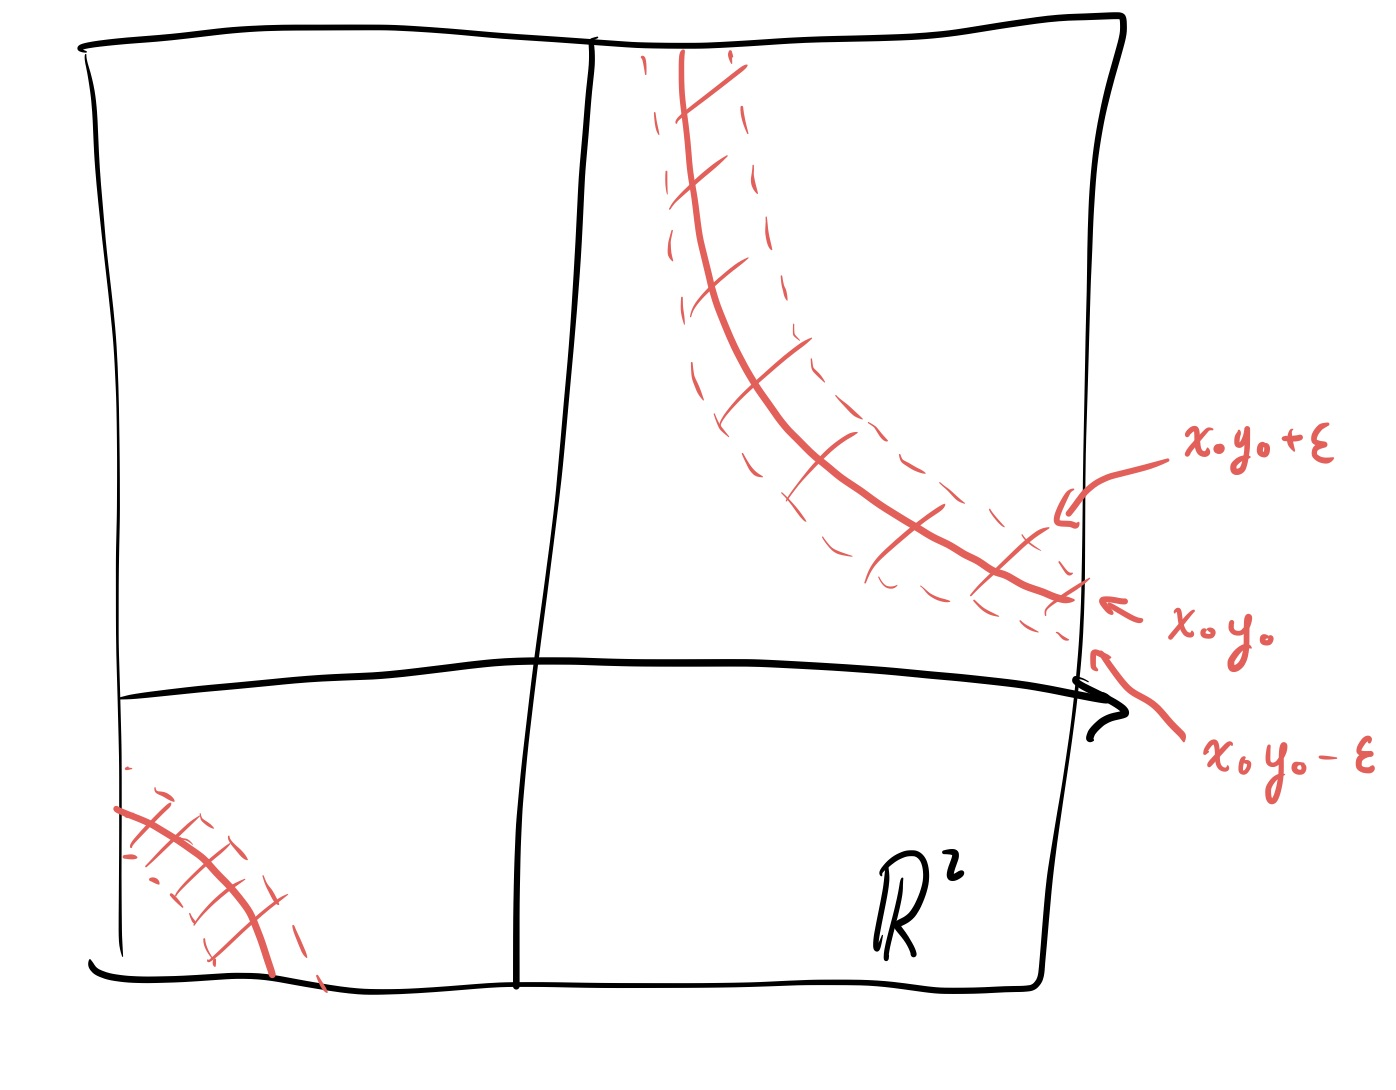
\includegraphics[width=.5\textwidth]{hw_3}
    \caption{Graph of a hyperbola and some tolerance \(\epsilon\).}
    \label{fig:Hyperbola}
  \end{figure}
  Let \(\delta = \frac{\epsilon}{|x_0| + |y_1| + 1}\). This proof went slightly awry in class, but was corrected in an email/canvas message later.
\end{proof}

\begin{df}
  Let \(\vec{x} \in \R^n\) \( r \in \R_{>0}\), the open ball of radius \(r\) centered at \(\vec{x}\) is the set
  \begin{align*}
    B(\vec{x}, r) = \opn \vec{y} \in \R^n\ :\ |\vec{x} - \vec{y}| < r\cls.
  \end{align*}
  A subset \(U \subseteq \R^n\) is called \textbf{open} if for each \(\vec{x} \in U\), there exists some \(\epsilon > 0\) such that \(B(\vec{x}, \epsilon) \subseteq U\).

  Let \(Z \subseteq \R^n\). A point \(\vec{x} \in \R^n\) is said to be a \textbf{limit point} of \(Z\) if \(B(\vec{x}, \epsilon) \cap Z \neq \emptyset\) for all \(\epsilon > 0\).

  A subset \(Z \subseteq \R^n\) is said to be closed if \(Z\) contains all of its limit points.
\end{df}

\begin{exa}
  
  \begin{enumerate}
  \item An open interval \((a, b) \subseteq \R\) is open and not closed
  \item A closed interval \([a,b] \subseteq \R\) is closed and not open
  \item The half open interval \([a, b) \subseteq \R\) is neither open nor closed
  \item \(\R \subseteq \R\) is neither.
  \end{enumerate}
\end{exa}

\begin{thm}
  A function \(f: \R^n \to \R^m\) is continuous iff for all open subsets \(U \subseteq \R^m\), \(f\1(u) \subseteq \R^n\) is an open subset of \(\R^n\).
\end{thm}
\end{document}
%%% Local Variables:
%%% mode: latex
%%% TeX-master: t
%%% End:




